\documentclass[12pt,letterpaper]{article}
\usepackage[utf8]{inputenc}
\usepackage[spanish]{babel}
\usepackage{graphicx}
\usepackage[left=2cm,right=2cm,top=2cm,bottom=2cm]{geometry}
\usepackage{graphicx} % figuras
% \usepackage{subfigure} % subfiguras
\usepackage{float} % para usar [H]
\usepackage{amsmath}
%\usepackage{txfonts}
\usepackage{stackrel} 
\usepackage{multirow}
\usepackage{enumerate} % enumerados
\renewcommand{\labelitemi}{$-$}
\renewcommand{\labelitemii}{$\cdot$}
% \author{}
% \title{Caratula}
\begin{document}

% Fancy Header and Footer
% \usepackage{fancyhdr}
% \pagestyle{fancy}
% \cfoot{}
% \rfoot{\thepage}
%

% \usepackage[hidelinks]{hyperref} % CREA HYPERVINCULOS EN INDICE

% \author{}
\title{Caratula}

\begin{titlepage}
\begin{center}
\large{UNIVERSIDAD PRIVADA DE TACNA}\\
\vspace*{-0.025in}
\begin{figure}[htb]
\begin{center}

\includegraphics[width=7cm]{./images/logo}
\end{center}
\end{figure}
\vspace*{0.15in}
INGENIERIA DE SISTEMAS  \\

\vspace*{0.3in}
\begin{large}
\textbf{TITULO:} \\
\end{large}

\vspace*{0.1in}
\begin{Large}
\textbf{Informe de Laboratorio Nº 04: Elaborando pruebas de una
aplicación Web
} \\

\end{Large}

\vspace*{0.3in}
\begin{Large}
\textbf{CURSO:} \\
\end{Large}

\vspace*{0.1in}
\begin{large}
Calidad y Pruebas de Software\\
\end{large}

\vspace*{0.3in}
\begin{Large}
\textbf{DOCENTE:} \\
\end{Large}

\vspace*{0.1in}
\begin{large}
 Ing. Patrick Cuadros Quiroga\\
\end{large}

\vspace*{0.4in}
\vspace*{0.1in}
\begin{large}
\textbf{INTEGRANTES:} \\
\begin{flushleft}
Yaneth Virginia Aquino Huallpa \hfill	(2017059286)\\

\centering  %CENTRA UN TEXTO
\vspace*{0.9in}
\begin{large}
Tacna
\end{large}

\end{flushleft}
\end{large}
\end{center}

\end{titlepage}


\section{Elaborando pruebas de una aplicación Web} 
\begin{itemize}
 \item  Crear el proyecto de prueba de .NET Core.
\begin{center}
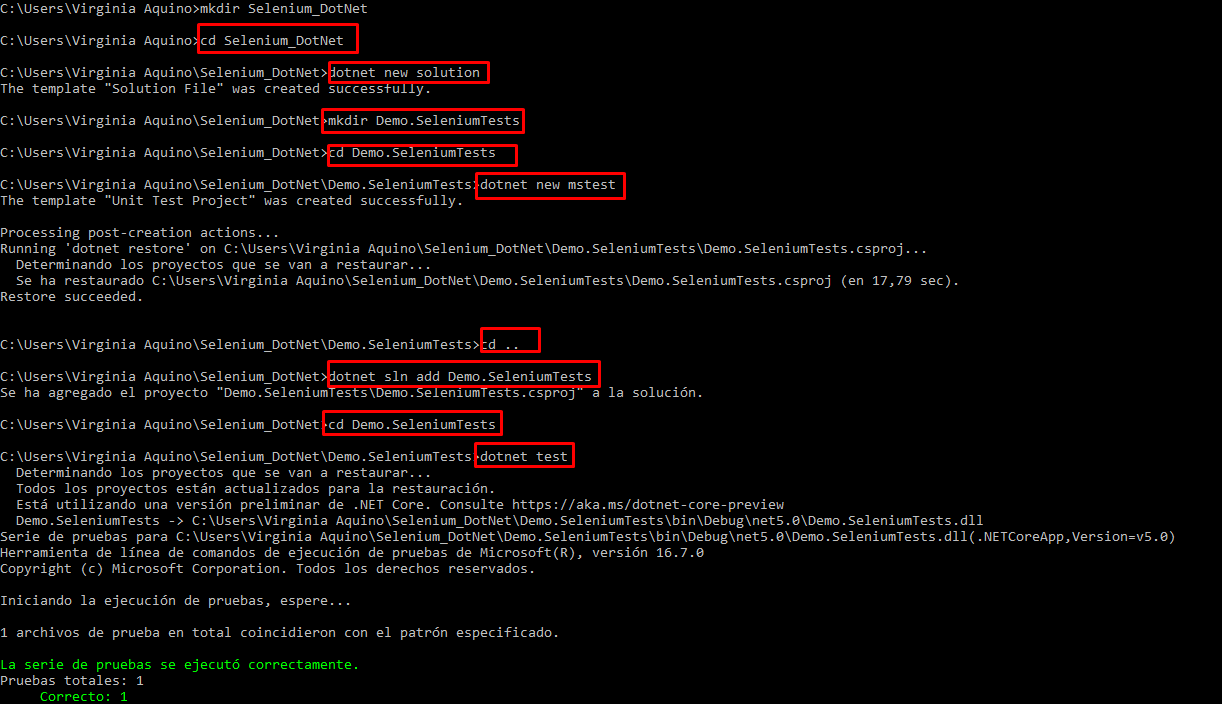
\includegraphics[width=\columnwidth]{images/1}\newline
\end{center}
\item Agregue Selenium al proyecto de prueba 
\begin{center}
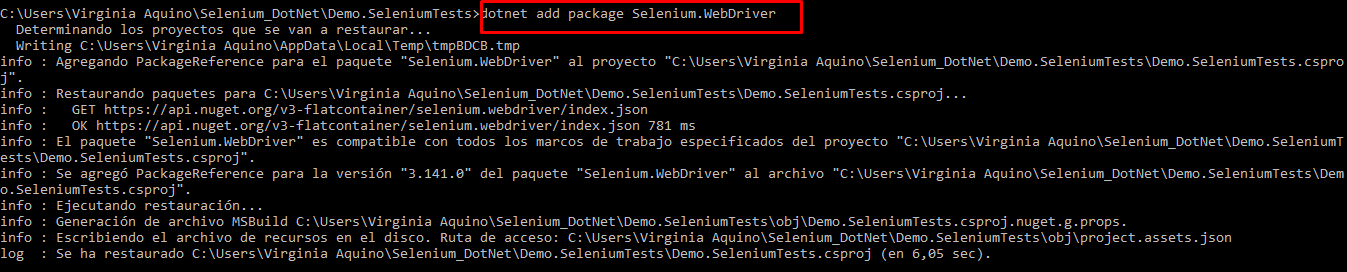
\includegraphics[width=\columnwidth]{images/2}\newline
\end{center}
\item Escriba una prueba de IU usando Selenium
\begin{center}
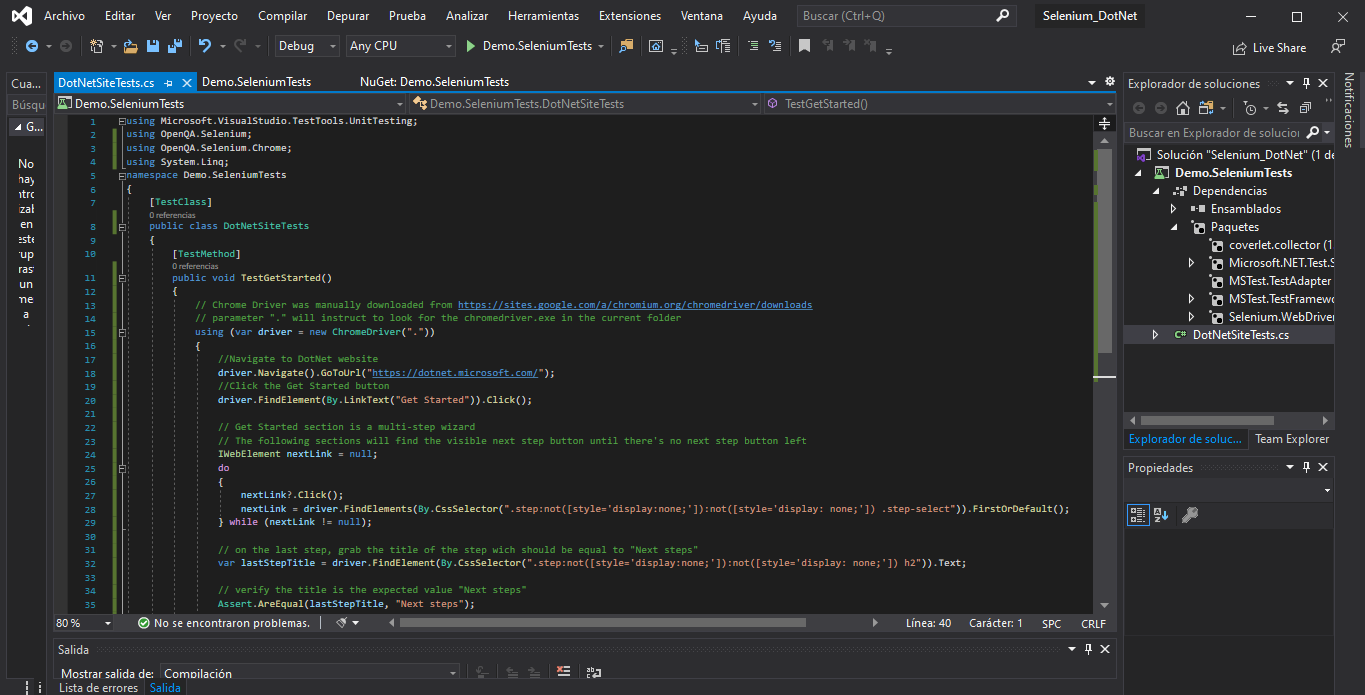
\includegraphics[width=\columnwidth]{images/3}\newline
\end{center}
\item Ejecute la prueba de IU
\begin{center}
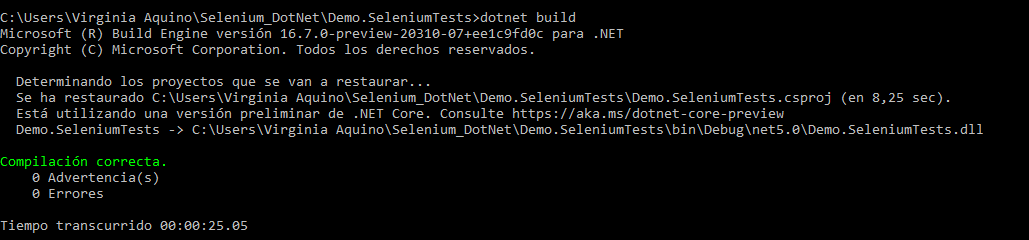
\includegraphics[width=\columnwidth]{images/4}\newline
\end{center}
\item Para Windows, puede usar este script de PowerShell:
\begin{center}
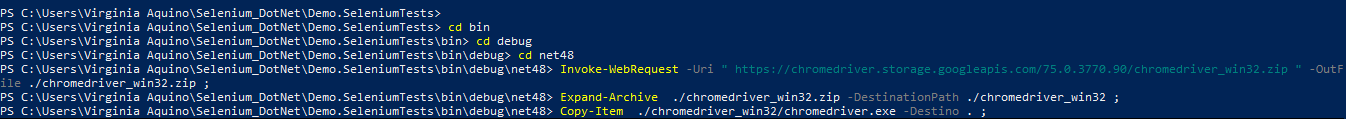
\includegraphics[width=\columnwidth]{images/5}\newline

\includegraphics[width=\columnwidth]{images/6}\newline
\end{center}
\item Solución de problemas: si la prueba falla debido a errores de Chrome / Chromium, siga estos pasos
Asegúrese de tener instalado Chrome / Chromium. descargar chrome version 75
\begin{center}
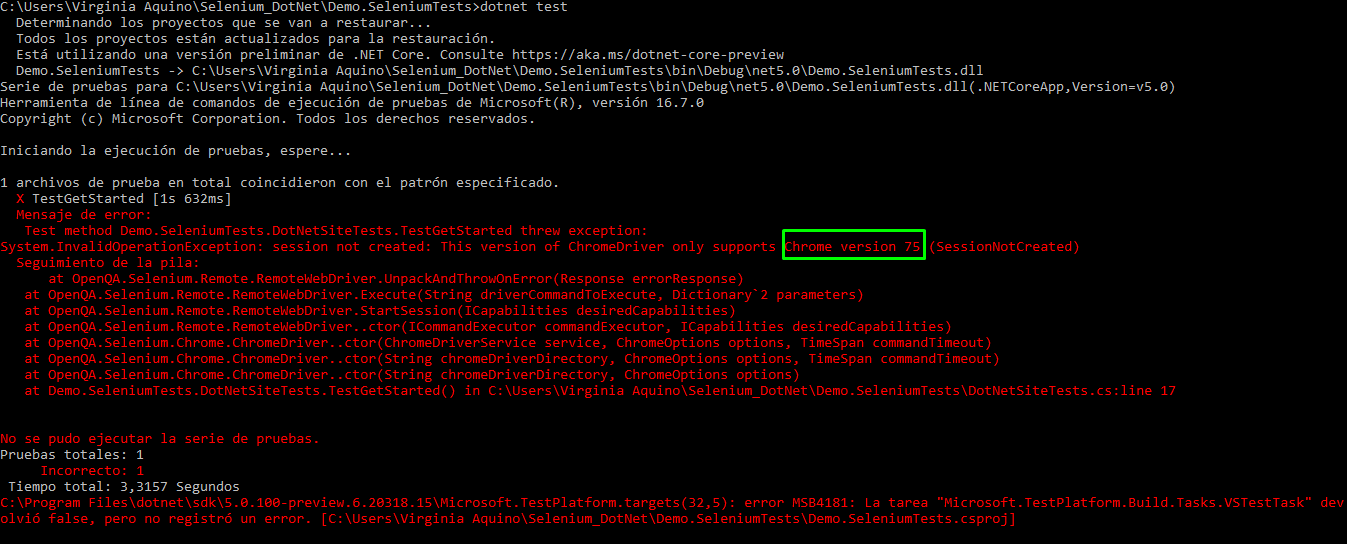
\includegraphics[width=\columnwidth]{images/error}\newline
\end{center}
\item Ejecute el comando de prueba dotnet
\begin{center}
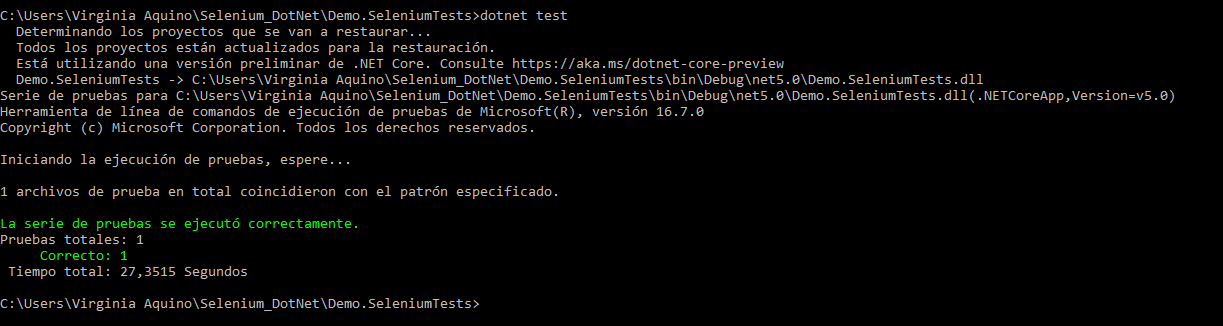
\includegraphics[width=\columnwidth]{images/final}\newline
\end{center}
\end{itemize}


\end{document}